% !TEX root = task-3-7-2.tex
% Editable task bank. Append new BankTask blocks at the end of the document.
\documentclass[12pt,a4paper]{article}
\usepackage{physics-textbook}
\usepackage{graphicx,needspace}
\usetikzlibrary{decorations.pathmorphing}
\newif\ifShowSolutions
\ifdefined\TutorEdition
  \ShowSolutionstrue
\else
  \ShowSolutionsfalse % Change to \ShowSolutionstrue to display solutions.
\fi
\newcounter{banktask}
\newsavebox{\BankTaskBox}
\newcommand{\BankTaskContent}[3]{%
  \noindent\textbf{\thebanktask.}\quad #2\par
  \ifShowSolutions
    \Needspace{50mm}% Keep the solution heading with its opening text or diagram.
    #3\par
    \ifdefined\TutorEdition
      \ifcsname TutorSource#1\endcsname
        \nopagebreak\smallskip{\small\csname TutorSource#1\endcsname\par}%
      \fi
    \fi
  \fi
}
\newcommand{\BankTask}[3]{%
  \refstepcounter{banktask}\par\medskip
  \sbox{\BankTaskBox}{\begin{minipage}{\linewidth}%
    \BankTaskContent{#1}{#2}{#3}\end{minipage}}%
  \ifdim\dimexpr\ht\BankTaskBox+\dp\BankTaskBox\relax>\dimexpr\textheight-20mm\relax
    \Needspace{35mm}\BankTaskContent{#1}{#2}{#3}%
  \else
    \Needspace{\dimexpr\ht\BankTaskBox+\dp\BankTaskBox\relax}%
    \noindent\usebox{\BankTaskBox}\par
  \fi
  \medskip
}
\begin{document}
\BookSubsection{3.7.2}{Ёмкость плоского конденсатора}


% Source sdamgia-6653: https://phys-ege.sdamgia.ru/problem?id=6653
\BankTask{sdamgia-6653}{
Плоский воздушный конденсатор заряжен до напряжения $U$. Площадь обкладок конденсатора $S$, расстояние между его пластинами $d$. Установите соответствие между физическими величинами и единицами их измерения.\par

\begin{center}\begin{minipage}[t]{.47\linewidth}\textbf{Физические величины}\par\smallskip А) Напряженность электрического поля в конденсаторе\par
Б) Емкость конденсатора\end{minipage}\hfill\begin{minipage}[t]{.47\linewidth}\textbf{Единицы измерения}\par\smallskip $1$. $\text{В/м}$\par
$2$. $\text{Дж}$\par
$3$. $\text{Кл/м}$\par
$4$. $\text{Ф}$\end{minipage}\end{center}
\par
\begin{center}\small\setlength{\tabcolsep}{3pt}\begin{tabular}{|p{0.45\linewidth}|p{0.45\linewidth}|}\hline
А & Б\\\hline
 & \\\hline
\end{tabular}\end{center}\par
}{
\smallskip\noindent\textbf{Решение}\par
Напряженность электрического поля измеряется в В/м. А емкость измеряется в фарадах.\par
Ответ: $14$.\par
}

% Source sdamgia-3191: https://phys-ege.sdamgia.ru/problem?id=3191
\BankTask{sdamgia-3191}{
Емкость плоского воздушного конденсатора равна $C$, напряжение между его обкладками $U$, расстояние между обкладками $d$. Чему равны заряд конденсатора и модуль напряженности электрического поля между его обкладками? Установите соответствие между физическими величинами и выражениями для них.\par

\begin{center}\begin{minipage}[t]{.47\linewidth}\textbf{Физическая величина}\par\smallskip А) Заряд конденсатора\par
Б) Модуль напряженности поля\end{minipage}\hfill\begin{minipage}[t]{.47\linewidth}\textbf{Выражение для нее}\par\smallskip $1$. $U/ ( 2d ) \;$\par
$2$. $CU ^2 /2\;$ \par
$3$. $CU$\par
$4$. $U/d\;$\end{minipage}\end{center}
\par
\begin{center}\small\setlength{\tabcolsep}{3pt}\begin{tabular}{|p{0.45\linewidth}|p{0.45\linewidth}|}\hline
$A$ & Б\\\hline
 & \\\hline
\end{tabular}\end{center}\par
}{
\smallskip\noindent\textbf{Решение}\par
Заряд конденсатора связан с его емкостью и напряжением между его обкладками соотношением $q=CU$ (А — $3$). Электрическое поле внутри плоского воздушного конденсатора однородное, и модуль его напряженности связан с напряжением на конденсаторе и расстоянием между пластинами соотношением $E= \frac{ U}{ d }$ (Б — $4$).\par
Ответ: $34$.\par
}

% Source sdamgia-9058: https://phys-ege.sdamgia.ru/problem?id=9058
\BankTask{sdamgia-9058}{
Модуль напряженности электрического поля в плоском воздушном конденсаторе емкостью $50 \,\text{мкФ}$ равен $200 \,\text{В/м}$. Расстояние между пластинами конденсатора $2 \,\text{мм}$. Чему равен заряд этого конденсатора? (В микрокулонах.)\par
}{
\smallskip\noindent\textbf{Решение}\par
Напряженность поля в конденсаторе может быть вычислена по формуле:\par
\[E= \frac{ U}{ d } \Longleftrightarrow U=Ed.\]
Заряд на обкладках конденсатора связан с емкостью и напряжением:\par
\[q=CU=CEd=50 \cdot 10 ^{ - 6 } \cdot 200 \cdot 2 \cdot 10 ^{ - 3 } =20\,\text{мкКл}.\]
Ответ: $20$.\par
}

% Source sdamgia-6930: https://phys-ege.sdamgia.ru/problem?id=6930
\BankTask{sdamgia-6930}{
На пластинах плоского воздушного конденсатора находятся электрические заряды +$q$ и -$q$. Площадь каждой пластины $S$, расстояние между ними $d$. Конденсатор отключен от источника. Как изменятся следующие физические величины: модуль напряженности поля в конденсаторе, емкость конденсатора, если увеличить расстояние между пластинами?\par
$1$. Увеличится.\par
$2$. Уменьшится.\par
$3$. Не изменится.\par
\begin{center}\small\setlength{\tabcolsep}{3pt}\begin{tabular}{|p{0.45\linewidth}|p{0.45\linewidth}|}\hline
Модуль напряженности поля
в конденсаторе & Емкость конденсатора\\\hline
 & \\\hline
\end{tabular}\end{center}\par
}{
\smallskip\noindent\textbf{Решение}\par
Поскольку конденсатор отключен от источника, заряд на его пластинах меняться не может. Формула для напряженности поля в конденсаторе: $E= \frac{ q}{ \varepsilon\varepsilon_{0}S } .$ Поскольку заряд на пластинах не изменился, то напряженность также не изменилась.\par
Емкость плоского конденсатора обратно пропорциональна расстоянию между пластинами: $C= \frac{ \varepsilon\varepsilon_{0}S}{ d } .$ Следовательно, при увеличении расстояния между его пластинами емкость уменьшится.\par
Ответ: $32$.\par
}

% Source sdamgia-19667: https://phys-ege.sdamgia.ru/problem?id=19667
\BankTask{sdamgia-19667}{
Площадь грозового облака $2 \,\text{км}^{2}$, напряженность электрического поля между облаком и землей $10^{6}\,\text{В/м}$. Считая, что облако и поверхность Земли образуют плоский конденсатор, найдите, чему равен модуль электрического заряда этого облака? (В кулонах и округлите до десятых долей.)\par
}{
\smallskip\noindent\textbf{Решение}\par
Напряженность электрического поля между поверхностью Земли и облаком равна $E= \frac{ U}{ d } .$ Заряд конденсатора равен $q = C \cdot U.$ Емкость плоского конденсатора равна $C= \frac{ \varepsilon _{0}S}{ d } .$ Отсюда получаем, что заряд равен\par
\[q = \frac{ Ed \varepsilon _{0}S}{ d } = E \varepsilon _{0}S = 10 ^{6} \cdot 8{,}85 \cdot 10 ^{ - 12 } \cdot 2 \cdot 10 ^{6} = 17{,}7\,\text{Кл}.\]
Ответ: $17{,}7$.\par
}

% Source sdamgia-12863: https://phys-ege.sdamgia.ru/problem?id=12863
\BankTask{sdamgia-12863}{
Плоский воздушный конденсатор, изготовленный из двух одинаковых квадратных металлических пластин, обладает электрической емкостью $96 \,\text{пФ}$. Каждую из пластин разрезали пополам вдоль стороны квадрата, собрали из получившихся прямоугольников два конденсатора и соединили их последовательно. Расстояние между пластинами конденсаторов оставили прежним. Определите электрическую емкость получившейся системы конденсаторов. (В пФ.)\par
}{
\smallskip\noindent\textbf{Решение}\par
Емкость плоского конденсатора равна $C= \frac{ \varepsilon\varepsilon_{0}S}{ d } .$ У получившихся прямоугольных конденсаторов площадь в два раза меньше исходной, и, значит, вдвое меньшая емкость — $48 \,\text{пФ}$. Емкость последовательно соединенных конденсаторов можно найти по формуле: $\frac{ 1}{ C_{0} } = \frac{ 1}{ C_{1} } + \frac{ 1}{ C_{2} } \Longleftrightarrow C_{0}= \frac{ C_{1}C_{2}}{ C_{1} + C_{2} } = \frac{ C_{1}}{ 2 } = \frac{ 48}{ 2 } = 24\,\text{пФ}.$\par
Ответ: $24$.\par
}

% Source sdamgia-8866: https://phys-ege.sdamgia.ru/problem?id=8866
\BankTask{sdamgia-8866}{
Плоский воздушный конденсатор, электроемкость которого равна $17{,}7 \,\text{пФ}$, заряжают до напряжения $5 \,\text{В}$ и отключают от источника напряжения. Затем одну пластину начинают медленно удалять от другой. Зависимость расстояния $d$ между пластинами от времени $t$ изображена на рисунке. Электрическая постоянная равна $\varepsilon_{0}=8{,}85\cdot10^{-12}\,\text{Ф/м}$.\par
$1$. Площадь поперечного сечения пластин конденсатора равна $20 \,\text{см}^{2}$.\par
$2$. Заряд на обкладках конденсатора уменьшается обратно пропорционально времени.\par
$3$. В момент времени $t=25 \,\text{с}$ электроемкость конденсатора станет равна $11{,}8 \,\text{пФ}$.\par
$4$. В момент времени $t=10 \,\text{с}$ напряженность электрического поля в конденсаторе равна $5 \,\text{кВ/м}$.\par
$5$. В момент времени $t=20 \,\text{с}$ напряжение между пластинами конденсатора равно $5 \,\text{В}$.\par

\begin{center}\begin{tikzpicture}[book diagram,>=stealth]
\draw[task grid,xstep=.1,ystep=.1](0,0)grid(5,4);\draw[task axis](0,0)--(5.3,0)node[right]{$t,\,\text{с}$};\draw[task axis](0,0)--(0,4.2)node[left]{$d,\,\text{мм}$};\foreach\x in{10,20,30,40}\node[below]at(\x/10,0){$\x$};\foreach\y/\s in{.8/.4,1.6/.8,2.4/1.2,3.2/1.6}\node[left]at(0,\y){$\s$};\node[below left]at(0,0){$0$};\draw[task curve](0,2)--(4.8,3.92);\foreach\x in{0,1,2,3,4}\fill(\x,{2+.4*\x})circle(1.5pt);
\end{tikzpicture}\end{center}
\par
}{
\smallskip\noindent\textbf{Решение}\par
Емкость плоского конденсатора находится по формуле:\par
\[C= \frac{ \varepsilon \varepsilon _{0} S}{ d } \Longleftrightarrow S= \frac{ Cd}{ \varepsilon \varepsilon _{0} } = \frac{ 17{,}7 \cdot 10 ^{ - 12 } \cdot 0{,}001}{ 1 \cdot 8{,}85 \cdot 10 ^{ - 12 } } =0{,}002\,\text{м} ^2 =20\,\text{см} ^2 ,\]
из чего следует, что утверждение $1$ верно.\par
Поскольку конденсатор отключили от источника тока, то заряд на его обкладках не меняется с течением времени (утверждение $2$ неверно) и равен $q=CU=17{,}7\,\text{пФ} \cdot 5\,\text{В}=88{,}5 \cdot 10 ^{ - 12 } \,\text{Кл}.$\par
В момент времени $t=25 \,\text{с}$ расстояние между обкладками равно $d =1{,}5\,\text{мм},$ тогда емкость конденсатора равна:\par
\[C= \frac{ \varepsilon \varepsilon _{0} S}{ d } = \frac{ 1 \cdot 8{,}85 \cdot 10 ^{ - 12 } \cdot 2 \cdot 10 ^{ - 3 } }{ 1{,}5 \cdot 10 ^{ - 3 } } =11{,}8\,\text{пФ},\]
а значит, утверждение $3$ верно.\par
Электрическое поле внутри конденсатора может быть найдено по формуле:\par
\[E= \frac{ U}{ d } = \frac{ q}{ Cd } .\]
Емкость конденсатора обратно пропорционально зависит от $d$, а значит, поле внутри конденсатора, отключенного от источника при изменении расстояния между пластинами не изменяется и равно:\par
\[E= \frac{ 88{,}5 \cdot 10 ^{ - 12 } }{ 17{,}7 \cdot 10 ^{ - 12 } \cdot 0{,}001 } =5\,\text{кВ/м},\]
а значит, утверждение $4$ верно.\par
В момент времени $t=20 \,\text{с}$ расстояние между обкладками равно $d =1{,}4\,\text{мм},$ тогда напряжение между пластинами конденсатора равно:\par
\[U=Ed=5\,\text{кВ/м} \cdot 1{,}4\,\text{мм} = 7\,\text{В},\]
а значит, утверждение $5$ неверно.\par
Ответ: $134$.\par
}

% Source sdamgia-7713: https://phys-ege.sdamgia.ru/problem?id=7713
\BankTask{sdamgia-7713}{
В плоский конденсатор, расстояние между обкладками которого равно $3 \,\text{см}$, вставили плоскопараллельную металлическую пластину толщиной $2{,}5 \,\text{см}$. Плоскости пластины параллельны обкладкам конденсатора, расстояние между обкладками намного меньше их поперечных размеров, пластина не касается обкладок. Во сколько раз в результате этого увеличилась электроемкость конденсатора?\par
}{
\smallskip\noindent\textbf{Решение}\par
Емкость плоского конденсатора пропорциональна диэлектрической проницаемости диэлектрика внутри него: $C= \frac{ \varepsilon\varepsilon_{0}S}{ d } .$\par
При любом положении параллельной пластины новая емкость $C_{1}$ будет одной и той же, соответствующей обычному конденсатору с расстоянием между пластинами, равному $d - b,$ где $d$ — расстояние между обкладками, а $b$ — толщина металлической пластины.\par
Поскольку $\frac{C_1}{C}=\frac{d}{d-b},$ то $C_{1}= \frac{ Cd}{ d - b } = \frac{ C \cdot 3}{ 3 - 2{,}5 } =6C.$ Таким образом, емкость конденсатора увеличится в $6$ раз.\par
Ответ: $6$.\par
}

% Source sdamgia-52050: https://phys-ege.sdamgia.ru/problem?id=52050
\BankTask{sdamgia-52050}{
Маленький шарик массой $m=0{,}4 \,\text{г}$, несущий заряд $q=5 \,\text{нКл}$, находится в равновесии между двумя горизонтальными пластинами плоского воздушного конденсатора ёмкостью $C=2 \,\text{нФ}$. Расстояние между обкладками конденсатора $d=1 \,\text{мм}$. Определите модуль заряда на обкладках конденсатора.\par
}{
\smallskip\noindent\textbf{Решение}\par
На шарик действуют сила тяжести и сила $F$ со стороны однородного электрического поля конденсатора. Так как шарик находится в равновесии, запишем второй закон Ньютона: $mg = F,$ где $F = E q,$ а $E$ — напряжённость электрического поля.\par
Модуль напряжённости электрического поля равен: $E = \frac{ U}{ d } ,$ где $U$ — напряжение между пластинами конденсатора. Выразим напряжение через модуль заряда пластины конденсатора и его электроёмкость: $U = \frac{ q_{k}}{ C } ,$ где $q_{k}$ — модуль заряда конденсатора, $C$ — электроёмкость конденсатора.\par
Тогда получим:\par
\[q_{k} = \frac{ C d g m}{ q } = \frac{ 2 \cdot 10 ^{ - 9 } \cdot 10 ^{ - 3 } \cdot 10 \cdot 0{,}4 \cdot 10 ^{ - 3 } }{ 5 \cdot 10 ^{ - 9 } } \approx 1{,}6 \cdot 10 ^{ - 6 } \,\text{Кл}.\]
Ответ: $q_{k} \approx 1{,}6 \cdot 10 ^{ - 6 } \,\text{Кл}.$\par
}

% Source sdamgia-29127: https://phys-ege.sdamgia.ru/problem?id=29127
\BankTask{sdamgia-29127}{
Обкладки плоского воздушного конденсатора изготовлены из двух тонких квадратных металлических пластин со стороной $a$ (на рисунке показан вид сбоку). Расстояние между обкладками $d\ll a$. Этот конденсатор подключен к источнику постоянного напряжения $U$ с пренебрежимо малым внутренним сопротивлением.\par
Через пространство между обкладками начинают медленно протаскивать с постоянной скоростью $V$ квадратную пластину со стороной $a$ и толщиной $d$, сделанную из однородного непроводящего материала с диэлектрической\par
проницаемостью $\varepsilon.$ В некоторый момент все пространство между обкладками конденсатора оказывается заполненным диэлектриком. Затем пластину продолжают двигать в том же направлении с той же скоростью до тех пор, пока она не покинет пространство между обкладками.\par
Опираясь на законы физики, изобразите график зависимости силы электрического тока $I$, протекающего через источник напряжения, от времени $t$. Искажениями электрического поля вблизи краев обкладок и пластины можно пренебречь. Отсчет времени начинается в момент, когда правый край пластины находится на уровне левых краев обкладок конденсатора, а заканчивается — когда пластина оказывается полностью вынутой из конденсатора с противоположной стороны. Объясните построение графика, указав явления и закономерности, которые Вы при этом использовали. На осях координат обозначьте физические величины в «особых» точках графика (максимумы, минимумы, разрывы, точки излома графика), если они есть.\par

\begin{center}\begin{tikzpicture}[book diagram,>=stealth]
\draw[very thick](0,0)--(4,0)(0,1)--(4,1);\draw[fill=orange!25](-2.8,.02)rectangle(1.2,.98);\node[above]at(-1.8,1){П};\node at(-.8,.5){$\mathcal E$};\draw[->](1.2,.5)--(1.9,.5)node[midway,above]{$V$};\node[font=\scriptsize]at(2.85,.5){конденсатор};\draw[<->](0,1.35)--(4,1.35)node[midway,above]{$a$};\draw[<->](3.9,.05)--(3.9,.95)node[midway,left]{$d$};\draw(4,1)--(5,1.3)--(5,.65)(5,.45)--(5,-.3)--(4,0);\draw[very thick](4.7,.65)--(5.3,.65)(4.85,.45)--(5.15,.45);\node[right]at(5.3,.55){$U$};
\end{tikzpicture}\end{center}
\par
}{
\smallskip\noindent\textbf{Решение}\par
$1$. Пусть правый край пластины находится внутри конденсатора на расстоянии $x$ от левых краев обкладок $( 0 \le x \le a ) .$ В этот момент времени $t$ можно представить рассматриваемый конденсатор как систему, состоящую из двух параллельно соединенных конденсаторов. Первый их них заполнен диэлектриком и имеет площадь обкладки $ax$, а второй — воздушный, с площадью обкладки $( a - x ) a.$\par
$2$. Емкость первого конденсатора равна $C_{1}= \frac{ \mathcal E_{0} \mathcal E ax}{ d } ,$ емкость второго конденсатора равна $C_{2}= \frac{ \mathcal E_{0} ( a - x ) a}{ d } .$ Здесь:\par
\[\mathcal E_{0}= \frac{ 1}{ 4 \pi k } \approx 8{,}85 \cdot 10 ^{ - 12 } \; \,\text{Ф}/\,\text{м}.\]
В соответствии с формулой для емкости параллельно соединенных конденсаторов, емкость рассматриваемого конденсатора в данный момент равна:\par
\[C=C_{1} + C_{2}= \frac{ \mathcal E_{0} a}{ d } ( ( \mathcal E - 1 ) x + a ) .\]
$3$. Заряд конденсатора в данный момент равен:\par
\[q=CU= \frac{ \mathcal E_{0} aU}{ d } ( ( \mathcal E - 1 ) x + a ) .\]
Поскольку пластина движется равномерно, то $x=Vt$:\par
\[q ( t ) =CU= \frac{ \mathcal E_{0} aU}{ d } ( ( \mathcal E - 1 ) Vt + a ) .\]
Следовательно, сила тока, текущего через источник, равна:\par
\[I= \frac{ \Delta q}{ \Delta t } = \frac{ \mathcal E_{0} aU ( \mathcal E - 1 ) V}{ d } =I_{0}=const.\]
Этот постоянный ток источника заряжает конденсатор, поскольку его емкость возрастает при вдвигании пластины в пространство между обкладками.\par
$4$. Полученный результат справедлив при:\par
\[0 \le t \le \frac{ a}{ V } .\]
В момент времени $t_{0}= \frac{ a}{ V }$ пластина займет все пространство между обкладками конденсатора, после чего начнет выходить наружу. Из соображений симметрии ясно, что при\par
\[\frac{ a}{ V } \le t \le \frac{ 2a}{ V }\]
через источник будет протекать точно такой же по модулю, но противоположный по знаку ток -$I_{0}$, поскольку емкость, а значит, и заряд конденсатора будут уменьшаться.\par

\begin{center}\begin{tikzpicture}[book diagram,>=stealth]
\draw[task axis](0,-1.6)--(0,1.7)node[above]{$I$};\draw[task axis](0,0)--(4.5,0)node[right]{$t$};\node[below left]at(0,0){$0$};\node[left]at(0,1){$I_0$};\node[left]at(0,-1){$-I_0$};\node[below left]at(2,0){$t_0$};\node[above]at(4,0){$2t_0$};\draw[task curve](0,0)--(0,1)--(2,1)--(2,-1)--(4,-1)--(4,0);\foreach\x in{0,2,4}\fill(\x,0)circle(1.5pt);
\end{tikzpicture}\end{center}
\par
$5$. График зависимости силы электрического тока $I$, протекающего через источник напряжения, от времени $t$ изображен на рисунке. Отметим, что в рамках рассматриваемой модели в определенные моменты времени сила тока изменяется скачкообразно: в момент $t=0$ — от $0$ до $I_{0}$; в момент $t=t_{0}= \frac{ a}{ V }$ — от $I_{0}$ до -$I_{0}$; в момент $t=2t_{0}= \frac{ 2a}{ V }$ — от -$I_{0}$ до $0$.\par
}


% Source 0A8805: https://ege.fipi.ru/bank/questions.php?search=1&proj=BA1F39653304A5B041B656915DC36B38&qid=0A8805
\BankTask{0A8805}{
Во сколько раз увеличится частота свободных электромагнитных колебаний в контуре, если площадь пластин конденсатора, входящего в состав контура, уменьшить в \(9\) раз, а индуктивность катушки увеличить в \(4\) раза?
}{
\smallskip\noindent\textbf{Решение от GPT}\par
Ёмкость конденсатора \(C=\varepsilon_0\varepsilon S/d\), поэтому \(C_2=C_1/9\). По формуле Томсона \(\nu=1/(2\pi\sqrt{LC})\), откуда
\[
\frac{\nu_2}{\nu_1}=\sqrt{\frac{L_1C_1}{(4L_1)(C_1/9)}}=\frac{3}{2}=1{,}5.
\]
Ответ: увеличится в \(1{,}5\) раза.
}

% Source 2786AC: https://ege.fipi.ru/bank/questions.php?search=1&proj=BA1F39653304A5B041B656915DC36B38&qid=2786AC
\BankTask{2786AC}{
В устройстве, изображённом на рисунке, лёгкий шарик из алюминиевой фольги подвешен между пластинами плоского конденсатора на изолирующей нити, при этом одна из пластин заземлена, а другая заряжена положительно. Когда устройство собрано, шарик приходит в колебательное движение, при котором сталкивается с пластинами конденсатора.

Какие утверждения соответствуют колебательному движению шарика в конденсаторе после первого столкновения шарика с пластиной?
\begin{enumerate}
\item Пренебрегая сопротивлением воздуха при движении шарика, его колебания можно считать гармоническими.
\item При движении шарика к заземлённой пластине он заряжен положительно, а при движении к положительно заряженной пластине -- отрицательно.
\item При движении шарика к положительно заряженной пластине его заряд равен нулю, а при движении к заземлённой пластине его заряд -- положительный.
\item По мере колебаний шарика электрическая ёмкость конденсатора увеличивается.
\item По мере колебаний шарика заряд конденсатора уменьшается.
\end{enumerate}
\begin{center}
\begin{tikzpicture}[book diagram,x=1cm,y=1cm,line cap=round,line join=round]
% Верхняя опора и подвес.
\fill[gray!60] (0.9,6.2) rectangle (3.45,6.32);
\draw[line width=1pt] (0.9,6.32)--(3.45,6.32);
\draw (2.18,6.2)--(2.18,3.16);
\shade[ball color=gray!25] (2.18,3.04) circle (0.16);
\draw (2.18,3.04) circle (0.16);
% Основание установки.
\draw[fill=gray!45] (0,0.72)--(3.95,0.72)--(4.06,0.9)--(3.95,1.08)--(0,1.08)--(0.1,0.9)--cycle;
% Изогнутые стойки.
\draw[fill=gray!55] (0.73,1.08)--(0.73,2.91) .. controls (0.73,3.12) and (0.87,3.19) .. (1.08,3.19)--(1.35,3.19)--(1.35,2.98)--(1.1,2.98) .. controls (1,2.98) and (0.95,2.94) .. (0.95,2.84)--(0.95,1.08)--cycle;
\draw[fill=gray!55] (3.48,1.08)--(3.48,2.91) .. controls (3.48,3.12) and (3.34,3.19) .. (3.13,3.19)--(2.88,3.19)--(2.88,2.98)--(3.11,2.98) .. controls (3.21,2.98) and (3.26,2.94) .. (3.26,2.84)--(3.26,1.08)--cycle;
% Крепления пластин.
\draw[fill=gray!75] (1.25,2.91) rectangle (1.49,3.25);
\draw[fill=gray!75] (2.88,2.91) rectangle (3.13,3.25);
% Пластины конденсатора.
\draw[fill=gray!15] (1.49,2.01) rectangle (1.55,4.04);
\draw[fill=gray!15] (2.83,2.01) rectangle (2.89,4.04);
\node at (1.28,3.94) {$+$};
% Зажимы на основании.
\foreach \x in {0.84,3.37}{
\draw[fill=gray!70] ({\x-0.23},0.64) rectangle ({\x+0.23},1.13);
\draw[fill=gray!65] ({\x-0.15},1.13) rectangle ({\x+0.15},1.32);
\draw[fill=black] ({\x-0.065},0.64)--({\x+0.065},0.64)--({\x+0.065},0.43)--({\x+0.17},0.35) .. controls ({\x+0.2},0.25) and ({\x-0.2},0.25) .. ({\x-0.17},0.35)--({\x-0.065},0.43)--cycle;
}
% Провод к земле.
\draw (2.89,3.8) .. controls (3.03,3.82) and (3.02,3.7) .. (3.2,3.72) .. controls (3.42,3.67) and (3.55,3.65) .. (3.65,3.47) .. controls (3.83,3.44) and (3.79,3.27) .. (3.93,3.18) .. controls (4.12,2.97) and (4.14,2.8) .. (4.28,2.64) .. controls (4.45,2.39) and (4.3,2.25) .. (4.4,2.12) .. controls (4.54,1.94) and (4.43,1.83) .. (4.53,1.68) .. controls (4.63,1.53) and (4.5,1.35) .. (4.61,1.2) .. controls (4.78,0.96) and (4.73,0.82) .. (4.87,0.59) .. controls (5.02,0.36) and (4.91,0.19) .. (4.91,0.03);
\draw (4.68,0.03)--(5.15,0.03);
\foreach \x in {4.7,4.78,4.86,4.94,5.02,5.1}{\draw (\x,0.03)--++(-0.1,-0.15);}
\end{tikzpicture}
\end{center}
}{
\smallskip\noindent\textbf{Решение от GPT}\par
При контакте с положительной пластиной шарик получает положительный заряд, а при контакте с заземлённой в поле конденсатора — отрицательный: утверждение 2 верно, а 3 неверно. Сила $\vec F=q\vec E$ не является возвращающей силой вида $F_x=-kx$, а столкновения меняют заряд шарика, поэтому колебания не гармонические и утверждение 1 неверно. Ёмкость $C=\varepsilon_0 S/d$ определяется геометрией конденсатора и не увеличивается: утверждение 4 неверно. Шарик переносит заряд между пластинами, разряжая конденсатор, поэтому утверждение 5 верно. Ответ: 2, 5.
}

% Source 0cDA83: https://ege.fipi.ru/bank/questions.php?search=1&proj=BA1F39653304A5B041B656915DC36B38&qid=0cDA83
\BankTask{0cDA83}{
Плоский воздушный конденсатор ёмкостью \(C_0\) состоит из двух металлических пластин, находящихся на расстоянии \(d_0\) друг от друга. Конденсатор зарядили и отключили от источника постоянного напряжения. Расстояние между пластинами меняется со временем так, как показано на графике.
\begin{enumerate}
\item В интервале времени от \(0\) до \(t_4\) ёмкость конденсатора остаётся неизменной.
\item В интервале времени от \(t_1\) до \(t_4\) заряд конденсатора остаётся неизменным.
\item В интервале времени от \(0\) до \(t_4\) энергия конденсатора уменьшается.
\item В интервале времени от \(0\) до \(t_4\) напряжённость электрического поля между пластинами конденсатора остаётся постоянной.
\item В интервале времени от \(0\) до \(t_4\) напряжение между пластинами конденсатора уменьшается.
\end{enumerate}
\begin{center}
\begin{tikzpicture}[book diagram,x=0.65cm,y=0.65cm]
\foreach \y in {1,...,5}{\draw[thin] (0.35,\y)--(2.35,\y);}
\foreach \x in {1,2}{\draw[thin] (\x,1.33)--(\x,4.67);}
\foreach \x in {3,4}{\draw[dashed,thin] (\x,0)--(\x,5);}
\draw[-{book tip}] (0,0)--(5.2,0) node[below] {$t$};
\draw[-{book tip}] (0,0)--(0,6) node[left] {$d$};
\node[below left] at (0,0) {$0$};
\foreach \i in {1,...,4}{\draw (\i,-0.12)--(\i,0.12);\node[below] at (\i,-0.12) {$t_{\i}$};}
\foreach \j in {1,...,5}{\draw (-0.12,\j)--(0.12,\j);}
\node[left] at (-0.12,1) {$d_0$};
\draw[very thick] (0,1)--(4,4);
\end{tikzpicture}
\end{center}
}{
\smallskip\noindent\textbf{Решение от GPT}\par
После отключения от источника заряд \(Q\) сохраняется, поэтому утверждение 2 верно. При увеличении \(d\) ёмкость \(C=\varepsilon_0S/d\) уменьшается, а энергия \(W=Q^2/(2C)\) увеличивается: утверждения 1 и 3 неверны. Поле \(E=Q/(\varepsilon_0S)\) постоянно, поэтому утверждение 4 верно. Напряжение \(U=Ed\) увеличивается, поэтому утверждение 5 неверно. Ответ: \(2,\ 4\).
}

% Source 675443: https://ege.fipi.ru/bank/questions.php?search=1&proj=BA1F39653304A5B041B656915DC36B38&qid=675443
\BankTask{675443}{
Плоский воздушный конденсатор ёмкостью \(C_0\), подключённый к источнику постоянного напряжения, состоит из двух металлических пластин, находящихся на расстоянии \(d_0\) друг от друга. Расстояние между пластинами меняется со временем так, как показано на графике.
\begin{enumerate}
\item В интервале времени от \(t_1\) до \(t_4\) заряд конденсатора возрастает.
\item В интервале времени от \(t_1\) до \(t_4\) энергия конденсатора равномерно уменьшается.
\item В промежутке времени от \(t_1\) до \(t_4\) напряжённость электрического поля между пластинами конденсатора остаётся постоянной.
\item В момент времени \(t_4\) ёмкость конденсатора увеличилась в $5$ раз по сравнению с первоначальной (при \(t=0\)).
\item В промежутке времени от \(t_1\) до \(t_4\) напряжённость электрического поля между пластинами конденсатора убывает.
\end{enumerate}
\begin{center}
\begin{tikzpicture}[book diagram,x=0.9cm,y=0.6cm]
\draw[thin] (0,0) grid[step=1] (4,6);
\draw[-{book tip}] (0,0)--(4.7,0) node[right] {$t$};
\draw[-{book tip}] (0,0)--(0,6.7) node[above] {$d$};
\node[below left] at (0,0) {$0$};
\node[left] at (0,5) {$d_0$};
\foreach \i in {1,...,4}{\node[below] at (\i,0) {$t_{\i}$};}
\draw[thick] (0,5)--(4,1);
\end{tikzpicture}
\end{center}
}{
\smallskip\noindent\textbf{Решение от GPT}\par
При постоянном напряжении $U$ расстояние $d$ уменьшается, поэтому $C=\varepsilon_0S/d$, $Q=CU$, $W=CU^2/2$ и $E=U/d$ возрастают. Утверждение 1 верно, утверждения 2, 3 и 5 неверны. По графику $d(t_4)=d_0/5$, следовательно, $C(t_4)=5C_0$: утверждение 4 верно. Ответ: $14$.
}

% Source 410957: https://ege.fipi.ru/bank/questions.php?search=1&proj=BA1F39653304A5B041B656915DC36B38&qid=410957
\BankTask{410957}{
Две параллельные металлические пластины больших размеров расположены на расстоянии \(d\) друг от друга и подключены к источнику постоянного напряжения (рис. 1). Пластины закрепили на изолирующих подставках и спустя длительное время отключили от источника (рис. 2).
\begin{enumerate}
\item Напряжённость электрического поля в точке \(B\) больше, чем в точке \(C\).
\item Потенциалы электрического поля в точках \(A\) и \(B\) одинаковы.
\item Если после отключения от источника увеличить расстояние \(d\) между пластинами, то напряжённость электрического поля в точке \(A\) увеличится.
\item Если после отключения от источника уменьшить расстояние \(d\) между пластинами, то заряд правой пластины не изменится.
\item Если после отключения от источника пластины полностью погрузить в керосин, то энергия электрического поля системы пластин уменьшится.
\end{enumerate}
\begin{center}
\begin{tikzpicture}[book diagram,x=0.8cm,y=0.8cm]
\draw[very thick] (0,0.7)--(0,3.5) (1.25,0.7)--(1.25,3.5);
\draw[thin] (0,3.5)--(0,4.35) (1.25,3.5)--(1.25,4.35);
\draw[{book tip}-{book tip}] (0,3.9)--(1.25,3.9) node[midway,above] {$d$};
\draw (0,1.85)--(-1.1,1.85)--(-1.1,-0.2)--(0.35,-0.2);
\draw (1.25,1.85)--(2.35,1.85)--(2.35,-0.2)--(0.9,-0.2);
\draw[fill=white] (0.35,-0.2) circle (0.065) (0.9,-0.2) circle (0.065);
\node[above] at (0.35,-0.15) {$-$};
\node[above] at (0.9,-0.15) {$+$};
\node at (0.625,-0.8) {Рис. 1};
\begin{scope}[xshift=4.7cm]
\draw[very thick] (0,0.7)--(0,3.5) (1.25,0.7)--(1.25,3.5);
\draw[thin] (0,3.5)--(0,4.35) (1.25,3.5)--(1.25,4.35);
\draw[{book tip}-{book tip}] (0,3.9)--(1.25,3.9) node[midway,above] {$d$};
\draw (0,1.85)--(-0.9,1.85) (1.25,1.85)--(2.15,1.85);
\fill (0.35,2.35) circle (0.045) node[above left] {$B$};
\fill (0.98,1.85) circle (0.045) node[above left] {$C$};
\fill (0.65,1.15) circle (0.045) node[left] {$A$};

\node at (0.625,-0.8) {Рис. 2};
\end{scope}
\end{tikzpicture}
\end{center}
}{
\smallskip\noindent\textbf{Решение от GPT}\par
Между большими параллельными пластинами поле однородно, поэтому \(E_B=E_C\) и утверждение 1 неверно. Точки \(A\) и \(B\) находятся на разных расстояниях от пластин, поэтому их потенциалы различаются: утверждение 2 неверно. После отключения заряд сохраняется, а \(E=Q/(\varepsilon_0S)\) не зависит от \(d\), поэтому утверждение 3 неверно, а 4 верно. При погружении в керосин ёмкость увеличивается в \(\varepsilon\) раз, а энергия \(W=Q^2/(2C)\) уменьшается в \(\varepsilon\) раз, поэтому утверждение 5 верно. Ответ: \(4,\ 5\).
}

% Source 82e66e: https://ege.fipi.ru/bank/questions.php?search=1&proj=BA1F39653304A5B041B656915DC36B38&qid=82e66e
\BankTask{82e66e}{
Ученику необходимо на опыте обнаружить зависимость электроёмкости плоского конденсатора от площади его пластин. У него имеется пять конденсаторов, характеристики которых приведены в таблице.

Какие два конденсатора необходимо взять ученику, чтобы провести данное исследование?

\begin{center}
\begin{tabular}{|c|c|c|c|}
\hline
\shortstack{№\\конденсатора} & \shortstack{Расстояние между\\пластинами, \(\text{мм}\)} & \shortstack{Площадь пластин,\\$\text{см}^{2}$} & \shortstack{Диэлектрик, заполняющий\\пространство между пластинами} \\
\hline
\(1\) & \(0{,}6\) & \(20\) & парафин \\
\hline
\(2\) & \(0{,}8\) & \(10\) & парафин \\
\hline
\(3\) & \(0{,}9\) & \(25\) & слюда \\
\hline
\(4\) & \(0{,}6\) & \(15\) & парафин \\
\hline
\(5\) & \(1{,}0\) & \(10\) & слюда \\
\hline
\end{tabular}
\end{center}
}{
\smallskip\noindent\textbf{Решение от GPT}\par
Электроёмкость плоского конденсатора $C=\varepsilon_0\varepsilon S/d$. Следует изменять площадь $S$, сохраняя расстояние $d$ и диэлектрик одинаковыми: этому условию соответствуют конденсаторы 1 и 4, у которых $d=0{,}6\,\text{мм}$, диэлектрик — парафин, а площади равны $20$ и $15\,\text{см}^2$. Ответ: 14.
}

% Source 19854: https://phys-ege.sdamgia.ru/problem?id=19854
\BankTask{19854}{
\begin{center}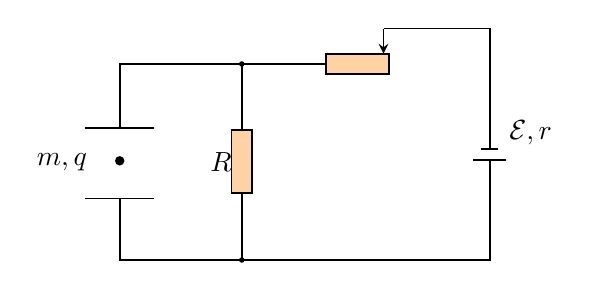
\begin{tikzpicture}[>=stealth,line width=.6pt]

\draw(0,1.17)--(0,1.98)--(2.62,1.98) (0,.27)--(0,-.51)--(4.7,-.51)--(4.7,.76)
 (4.7,.90)--(4.7,2.43)--(3.35,2.43);
\draw[->](3.35,2.43)--(3.35,2.11);
\draw(-.44,1.17)--(.44,1.17) (-.44,.27)--(.44,.27);
\draw(1.55,1.98)--(1.55,1.14) (1.55,.34)--(1.55,-.51);
\fill(0,.75)circle(.06) (1.55,1.98)circle(.035) (1.55,-.51)circle(.035);
\begin{scope}[shift={(3.02,1.98)},rotate=0]\draw[fill=orange!35] (-.4,-.13) rectangle (.4,.13);\end{scope}\begin{scope}[shift={(1.55,0.74)},rotate=90]\draw[fill=orange!35] (-.4,-.13) rectangle (.4,.13);\end{scope}\node[left] at (1.55,0.74) {$R$};\begin{scope}[shift={(4.7,0.83)},rotate=90]\draw(-.07,-.21)--(-.07,.21) (.07,-.11)--(.07,.11);\end{scope}\node[above right] at (4.82,0.83) {$\mathcal E,r$};\node[left]at(-.29,.73){$m,q$};
\end{tikzpicture}\end{center}
Две параллельные металлические пластины, расположенные горизонтально, подключены к электрической схеме, приведенной на рисунке. Между пластинами находится в равновесии маленькое заряженное тело массой m и зарядом q. Электростатическое поле между пластинами считать однородным. Опираясь на законы механики и электродинамики, объясните, как и в какую сторону начнет двигаться тело, если сдвинуть ползунок реостата влево.
}{
\smallskip\noindent\textbf{Решение}\par
\begin{center}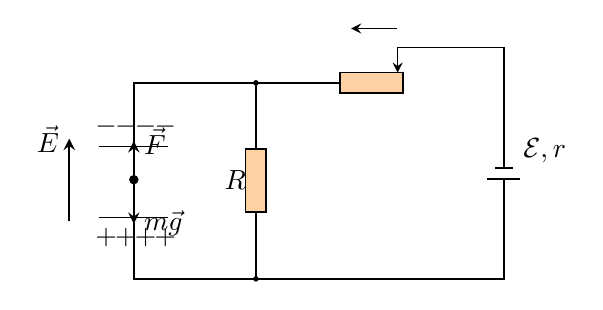
\begin{tikzpicture}[>=stealth,line width=.6pt]

\draw(0,1.17)--(0,1.98)--(2.62,1.98) (0,.27)--(0,-.51)--(4.7,-.51)--(4.7,.76)
 (4.7,.90)--(4.7,2.43)--(3.35,2.43);
\draw[->](3.35,2.43)--(3.35,2.11);
\draw(-.44,1.17)--(.44,1.17) (-.44,.27)--(.44,.27);
\draw(1.55,1.98)--(1.55,1.14) (1.55,.34)--(1.55,-.51);
\fill(0,.75)circle(.06) (1.55,1.98)circle(.035) (1.55,-.51)circle(.035);
\begin{scope}[shift={(3.02,1.98)},rotate=0]\draw[fill=orange!35] (-.4,-.13) rectangle (.4,.13);\end{scope}\begin{scope}[shift={(1.55,0.74)},rotate=90]\draw[fill=orange!35] (-.4,-.13) rectangle (.4,.13);\end{scope}\node[left] at (1.55,0.74) {$R$};\begin{scope}[shift={(4.7,0.83)},rotate=90]\draw(-.07,-.21)--(-.07,.21) (.07,-.11)--(.07,.11);\end{scope}\node[above right] at (4.82,0.83) {$\mathcal E,r$};
\foreach \x in {-.35,-.1,.15,.4}{\node at(\x,1.43){$-$};\node at(\x,.02){$+$};}
\draw[->,thick] (0,.75)--(0,.19)node[right]{$m\vec g$};
\draw[->,thick] (0,.75)--(0,1.24)node[right]{$\vec F$};
\draw[->,thick](-.82,.23)--(-.82,1.27)node[left]{$\vec E$};
\draw[->](3.34,2.67)--(2.76,2.67);

\end{tikzpicture}\end{center}
$1$.  Поскольку пластины подключены к источнику ЭДС, то между ними имеется разность потенциалов, в пространстве между ними создается однородное электростатическое поле. Согласно электрической схеме, нижняя пластина имеет положительный заряд, а верхняя  — отрицательный; следовательно, вектор напряженности поля направлен вертикально вверх. По условию задачи заряженное тело находится в равновесии; следовательно, сила тяжести скомпенсирована силой Кулона, направленной вертикально вверх. Отсюда делаем вывод, что тело имеет положительный заряд.
$2$.  Если сдвинуть ползунок реостата влево, то сопротивление реостата уменьшится. Поскольку реостат соединен с резистором R последовательно, то и общее сопротивление цепи также уменьшится. 
$3$.  Согласно закону Ома для полной цепи $\mathcal{E}=I ( R_{\,\text{цепи}} + r )$  — при уменьшении сопротивления внешней цепи сила тока в ней увеличится. Таким образом, по закону Ома для участка цепи цепи $U=IR$  — напряжение на резисторе R также увеличится. Поскольку пластины соединены с резистором R параллельно, то, соответственно, напряжение между ними увеличится. Следовательно, увеличится и напряженность поля между пластинами: $E=U/d.$
$4$.  Увеличение напряженности поля приведет к увеличению силы Кулона, действующей на тело: $F=qE.$ Равновесие нарушится, сила Кулона станет больше силы тяжести, и тело начнет двигаться вверх с ускорением.
}

% Source 29732: https://phys-ege.sdamgia.ru/problem?id=29732
\BankTask{29732}{
Воспользовавшись оборудованием, представленным на левом рисунке, учитель собрал модель плоского конденсатора (см. средний рис.), зарядил нижнюю пластину положительным зарядом, а корпус электрометра заземлил. Соединенная с корпусом электрометра верхняя пластина конденсатора приобрела отрицательный заряд, равный по модулю заряду нижней пластины. После этого учитель сместил одну пластину относительно другой не изменяя расстояния между ними (см. правый рис.). Как изменились при этом показания электрометра (увеличились, уменьшились, остались прежними)? Ответ поясните, указав, какие явления и закономерности вы использовали для объяснения. Показания электрометра в данном опыте прямо пропорциональны разности потенциалов между пластинами конденсатора.

\begin{center}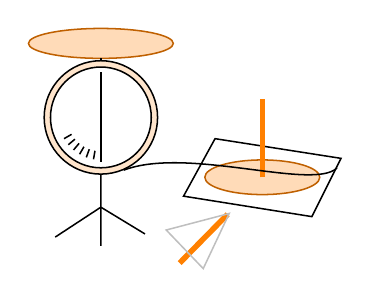
\begin{tikzpicture}[>=stealth,line width=.55pt]\draw[fill=orange!20](0,0)circle(.72);\draw[fill=white](0,0)circle(.64);\draw(0,-.72)--(0,-1.14)--(-.58,-1.52) (0,-1.14)--(.56,-1.48) (0,-1.14)--(0,-1.63);\foreach \a in {210,220,...,270}{\draw(\a:.43)--(\a:.54);}\draw(0,-.56)--(0,.58);\draw[thick](0,0)--(270:.56);\filldraw[fill=orange!28,draw=orange!75!black](0,.94)ellipse(.92 and .19);\draw(0,.75)--(0,.72);\begin{scope}[shift={(2.05,-.76)}]\draw(-1,-.24)--(.63,-.5)--(1,.24)--(-.6,.49)--cycle;\filldraw[fill=orange!28,draw=orange!75!black](0,0)ellipse(.73 and .22);\draw[orange,line width=2pt](0,0)--(0,1);\end{scope}\draw(.29,-.67) .. controls (1.1,-.36) and (2.7,-.94) .. (3,-.64);\draw[orange,line width=2pt](1,-1.85)--(1.61,-1.23);\draw[gray!50](.83,-1.43)--(1.63,-1.22)--(1.3,-1.92)--cycle;\end{tikzpicture}\end{center}

\begin{center}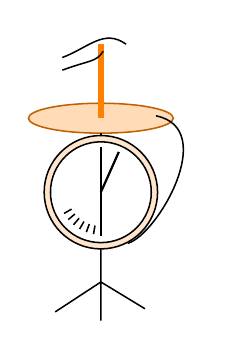
\begin{tikzpicture}[>=stealth,line width=.55pt]\draw[fill=orange!20](0,0)circle(.72);\draw[fill=white](0,0)circle(.64);\draw(0,-.72)--(0,-1.14)--(-.58,-1.52) (0,-1.14)--(.56,-1.48) (0,-1.14)--(0,-1.63);\foreach \a in {210,220,...,270}{\draw(\a:.43)--(\a:.54);}\draw(0,-.56)--(0,.58);\draw[thick](0,0)--(66:.56);\filldraw[fill=orange!28,draw=orange!75!black](0,.94)ellipse(.92 and .19);\draw(0,.75)--(0,.72);\draw[orange,line width=2pt](0,.94)--(0,1.88);\draw(.32,1.88)..controls(.04,2.08)and(-.15,1.84)..(-.49,1.71) (-.49,1.55)..controls(-.14,1.68)and(-.06,1.65)..(.03,1.79);\draw(.7,.97)..controls(1.5,.81)and(.72,-.54)..(.34,-.65);\end{tikzpicture}\end{center}

\begin{center}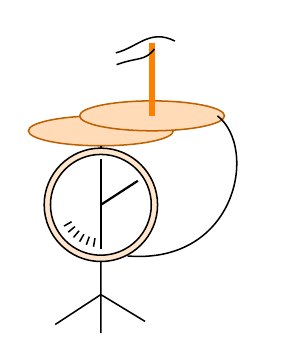
\begin{tikzpicture}[>=stealth,line width=.55pt]\draw[fill=orange!20](0,0)circle(.72);\draw[fill=white](0,0)circle(.64);\draw(0,-.72)--(0,-1.14)--(-.58,-1.52) (0,-1.14)--(.56,-1.48) (0,-1.14)--(0,-1.63);\foreach \a in {210,220,...,270}{\draw(\a:.43)--(\a:.54);}\draw(0,-.56)--(0,.58);\draw[thick](0,0)--(33:.56);\filldraw[fill=orange!28,draw=orange!75!black](0,.94)ellipse(.92 and .19);\draw(0,.75)--(0,.72);\filldraw[fill=orange!28,draw=orange!75!black](.65,1.13)ellipse(.92 and .19);\draw[orange,line width=2pt](.65,1.13)--(.65,2.05);\draw(.94,2.08)..controls(.62,2.24)and(.47,2)..(.19,1.93) (.2,1.78)..controls(.47,1.88)and(.56,1.82)..(.68,1.98);\draw(1.48,1.13)..controls(2,.73)and(1.73,-.76)..(.34,-.65);\end{tikzpicture}\end{center}
}{
\smallskip\noindent\textbf{Решение}\par
$1$.  При зарядке нижней пластины конденсатора стрежень и стрелка электрометра зарядятся одноименно с этой пластиной положительным зарядом. Соответственно, пластина, соединенная с корпусом получит отрицательный заряд. Данная система является замкнутой, поэтому в ней выполняется закон сохранения заряда. 
$2$.  При уменьшении общей площади пластин конденсатора уменьшится его емкость, исходя из формулы $C= \frac{\varepsilon \varepsilon_0 S}{d} .$ 
$3$.  Так как заряд на конденсаторе не изменился, его емкость уменьшилась, то разность потенциалов между его пластинами, исходя из формулы $C= \frac{q}{U} ,$ увеличилась. Соответственно, увеличилась разность потенциалов на электрометре. По условию угол отклонения стрелки электрометра пропорционален разности потенциалов. Следовательно, угол отклонения стрелки электрометра увеличился. 

Ответ: угол отклонения увеличится.
}

% Source 29730: https://phys-ege.sdamgia.ru/problem?id=29730
\BankTask{29730}{
\begin{center}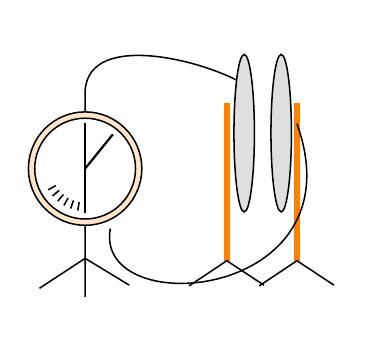
\begin{tikzpicture}[>=stealth,line width=.55pt]\draw[fill=orange!20](0,0)circle(.72);\draw[fill=white](0,0)circle(.64);\draw(0,-.72)--(0,-1.14)--(-.58,-1.52) (0,-1.14)--(.56,-1.48) (0,-1.14)--(0,-1.63);\foreach \a in {210,220,...,270}{\draw(\a:.43)--(\a:.54);}\draw(0,-.56)--(0,.58);\draw[thick](0,0)--(51:.56);\draw(0,.72)--(0,.99)..controls(.05,1.78)and(1.62,1.34)..(2.03,1.06);\draw[fill=gray!25](2.02,.45)ellipse(.13 and 1);\draw[fill=gray!25](2.49,.45)ellipse(.13 and 1);\foreach \x in {1.8,2.69}{\draw[orange,line width=2pt](\x,-1.17)--(\x,.83);\draw(\x,-1.17)--++(-.48,-.32) (\x,-1.17)--++(.47,-.31);}\draw(.32,-.76)..controls(.1,-1.95)and(3.5,-1.69)..(2.69,.57);\end{tikzpicture}\end{center} Две плоские пластины конденсатора, закрепленные на изолирующих штативах, расположили на небольшом расстоянии друг от друга и соединили одну пластину с заземленным корпусом, а другую  — со стержнем электрометра (см. рисунок). Затем пластину, соединенную со стержнем электрометра, зарядили. Объясните, опираясь на известные Вам законы, как изменяются показания электрометра при сближении пластин. Отклонение стрелки электрометра пропорционально разности потенциалов между пластинами. Емкость электрометра пренебрежимо мала.
}{
\smallskip\noindent\textbf{Решение}\par
$1$.  При зарядке левой пластины конденсатора стрежень и стрелка электрометра зарядятся одноименно с этой пластиной. Поскольку корпус электрометра заземлен, то на второй пластине конденсатора образуется заряд противоположного знака. Пластина со стержнем образуют замкнутую систему, поэтому в ней выполняется закон сохранения заряда. 
$2$.  При уменьшении расстояния между пластинами конденсатора увеличится его емкость, исходя из формулы $C= \frac{\varepsilon \varepsilon_0 S}{d} .$ 
$3$.  Так как заряд на конденсаторе не изменился, его емкость увеличилась, то разность потенциалов между его пластинами, исходя из формулы $C= \frac{q}{U} ,$ уменьшилась. Соответственно, уменьшилась разность потенциалов на электрометре. По условию угол отклонения стрелки электрометра пропорционален разности потенциалов. Следовательно, угол отклонения стрелки электрометра уменьшился. 

Ответ: угол отклонения уменьшится.
}

% Source 7873: https://phys-ege.sdamgia.ru/problem?id=7873
\BankTask{7873}{
Воспользовавшись оборудованием, представленным на рис. $1$, учитель собрал модель плоского конденсатора (рис. $2$), зарядил нижнюю пластину положительным зарядом, а корпус электрометра заземлил. Соединенная с корпусом электрометра верхняя пластина конденсатора приобрела отрицательный заряд, равный по модулю заряду нижней пластины. После этого учитель сместил одну пластину относительно другой не изменяя расстояния между ними (рис. $3$). Как изменились при этом показания электрометра (увеличились, уменьшились, остались прежними)? Ответ поясните, указав, какие явления и закономерности вы использовали для объяснения. Показания электрометра в данном опыте прямо пропорциональны разности потенциалов между пластинами конденсатора.

\begin{center}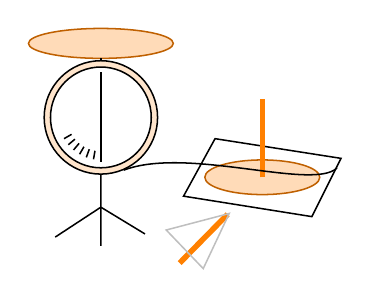
\begin{tikzpicture}[>=stealth,line width=.55pt]\draw[fill=orange!20](0,0)circle(.72);\draw[fill=white](0,0)circle(.64);\draw(0,-.72)--(0,-1.14)--(-.58,-1.52) (0,-1.14)--(.56,-1.48) (0,-1.14)--(0,-1.63);\foreach \a in {210,220,...,270}{\draw(\a:.43)--(\a:.54);}\draw(0,-.56)--(0,.58);\draw[thick](0,0)--(270:.56);\filldraw[fill=orange!28,draw=orange!75!black](0,.94)ellipse(.92 and .19);\draw(0,.75)--(0,.72);\begin{scope}[shift={(2.05,-.76)}]\draw(-1,-.24)--(.63,-.5)--(1,.24)--(-.6,.49)--cycle;\filldraw[fill=orange!28,draw=orange!75!black](0,0)ellipse(.73 and .22);\draw[orange,line width=2pt](0,0)--(0,1);\end{scope}\draw(.29,-.67) .. controls (1.1,-.36) and (2.7,-.94) .. (3,-.64);\draw[orange,line width=2pt](1,-1.85)--(1.61,-1.23);\draw[gray!50](.83,-1.43)--(1.63,-1.22)--(1.3,-1.92)--cycle;\end{tikzpicture}\end{center}
Рис. $1$

\begin{center}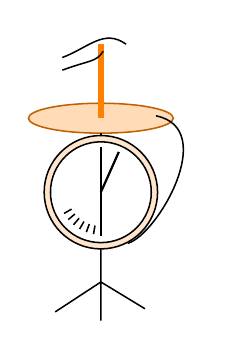
\begin{tikzpicture}[>=stealth,line width=.55pt]\draw[fill=orange!20](0,0)circle(.72);\draw[fill=white](0,0)circle(.64);\draw(0,-.72)--(0,-1.14)--(-.58,-1.52) (0,-1.14)--(.56,-1.48) (0,-1.14)--(0,-1.63);\foreach \a in {210,220,...,270}{\draw(\a:.43)--(\a:.54);}\draw(0,-.56)--(0,.58);\draw[thick](0,0)--(66:.56);\filldraw[fill=orange!28,draw=orange!75!black](0,.94)ellipse(.92 and .19);\draw(0,.75)--(0,.72);\draw[orange,line width=2pt](0,.94)--(0,1.88);\draw(.32,1.88)..controls(.04,2.08)and(-.15,1.84)..(-.49,1.71) (-.49,1.55)..controls(-.14,1.68)and(-.06,1.65)..(.03,1.79);\draw(.7,.97)..controls(1.5,.81)and(.72,-.54)..(.34,-.65);\end{tikzpicture}\end{center}
Рис. $2$

\begin{center}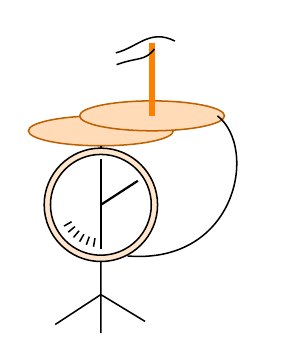
\begin{tikzpicture}[>=stealth,line width=.55pt]\draw[fill=orange!20](0,0)circle(.72);\draw[fill=white](0,0)circle(.64);\draw(0,-.72)--(0,-1.14)--(-.58,-1.52) (0,-1.14)--(.56,-1.48) (0,-1.14)--(0,-1.63);\foreach \a in {210,220,...,270}{\draw(\a:.43)--(\a:.54);}\draw(0,-.56)--(0,.58);\draw[thick](0,0)--(33:.56);\filldraw[fill=orange!28,draw=orange!75!black](0,.94)ellipse(.92 and .19);\draw(0,.75)--(0,.72);\filldraw[fill=orange!28,draw=orange!75!black](.65,1.13)ellipse(.92 and .19);\draw[orange,line width=2pt](.65,1.13)--(.65,2.05);\draw(.94,2.08)..controls(.62,2.24)and(.47,2)..(.19,1.93) (.2,1.78)..controls(.47,1.88)and(.56,1.82)..(.68,1.98);\draw(1.48,1.13)..controls(2,.73)and(1.73,-.76)..(.34,-.65);\end{tikzpicture}\end{center}
Рис. $3$
}{
\smallskip\noindent\textbf{Решение}\par
Стрелка и стержень, соединенные с пластиной, но изолированные от корпуса электрометра, заряжаются положительно, в результате взаимодействия стрелка отклоняется на некоторый угол.
Нижняя пластина создает вокруг себя электрическое поле, под действием которого в верхней пластине и металлическом корпусе электрометра происходит перераспределение зарядов, которое длится до тех пор, пока поверхности пластин не станут эквипотенциальными. В результате перераспределения зарядов верхняя пластинка заряжается отрицательно. Таким образом, заряды пластин становятся одинаковыми по модулю, но противоположными по знаку.
Система из двух заряженных пластин образует конденсатор емкостью $C = \frac{\,\text{эпсилон} \,\text{эпсилон} _0S}{d} .$ Поскольку расстояние между пластинами d и диэлектрическая проницаемость воздуха $\,\text{эпсилон}$ не изменились, а перекрываемая площадь пластин S уменьшилась, то и емкость конденсатора уменьшилась.
С другой стороны емкость конденсатора равна $C= \frac{q}{U} .$ Поскольку заряд на пластинах конденсатора остается постоянным, емкость уменьшается, то разность потенциалов между обкладками конденсатора увеличивается.
По условию задачи разность потенциалов пропорциональна показаниям электрометра, то при увеличении напряжения увеличивается угол отклонения стрелки. Показания электрометра увеличились.
}

\end{document}
